\documentclass[conference]{IEEEtran}
\usepackage{graphicx}
\usepackage{amsmath}
\usepackage{array}
\usepackage{multirow}
\usepackage{textcomp}
\usepackage{xcolor}

\newcommand{\pt}{\,pt}

\begin{document}

\title{Reconstructing and Re-Evaluating BSFR-SH:\\A Blockchain-Enabled Ransomware Defense Framework}

\author{
\IEEEauthorblockN{Course Project Report}
\IEEEauthorblockA{Reproduction study of Wazid, Das \& Shetty, \emph{IEEE Trans. Consumer Electronics}, 69(1):18--28, Feb.\ 2023}
}

\maketitle

\begin{abstract}
BSFR-SH claims a blockchain-protected, honeypot-driven detection and recovery framework for
ransomware in smart healthcare, reporting 98.98\% accuracy and 0.990 F1 on the BitcoinHeist
dataset. We built a complete, from-scratch implementation of all five of its algorithms, both
of its private blockchains under real pBFT consensus, and the honeypot feature pipeline the
paper specifies but never defines. Reproducing the paper's own evaluation protocol, our best
model reaches 0.9442 accuracy / 0.9697 F1 -- 4.56 points below the published figure, and an
ablation over both candidate leakage sources we identified narrows but does not close a
3.58-point residual gap. We further
identify five independent defects spanning the paper's evaluation methodology, security
argument, and preprocessing specification. The framework's central idea -- chain-protecting a
detector's ground truth and a system's backups from the same adversary -- is sound; several of
the paper's supporting claims measurably are not.
\end{abstract}

\section{Introduction}

BSFR-SH \cite{wazid2023} proposes a blockchain-enabled defense against ransomware for smart
healthcare networks. Its contribution is architectural: two independent, permissioned
blockchains, one holding encrypted data backups and one holding ransomware signatures and
behavioural features harvested from a honeypot, both committed through pBFT consensus among a
fixed set of cloud servers. The pitch is that an attacker who compromises a protected system
cannot also tamper with the detector's ground truth or destroy the means of recovery, because
both are chain-certified and the chain is Byzantine-fault-tolerant against a minority of
colluding servers. On top of this architecture the paper reports a ransomware detector that
reaches 98.98\% accuracy and 0.990 F1 on the BitcoinHeist dataset, beating four prior published
detectors, and a consensus/backup pipeline that commits 1500 transactions in under seven
seconds.

No artifact accompanies the paper: no code, no declared hyperparameters, no train/test protocol
beyond ``90/10,'' no definition of what a honeypot-derived ``signature'' or ``feature'' actually
is. Reproducing a paper under those conditions means first building the thing it describes
closely enough that its own claims become checkable, and only then checking them. This report
does both. We built the full system -- crypto layer, two blockchains, pBFT consensus, honeypot
sample synthesis and feature extraction, a dual-backend ML detection module, a mitigation state
machine, and a recovery path -- against the paper's own algorithm listings, and we ran its own
evaluation protocol wherever the paper specifies one. Where it does not -- which, as
\S\ref{sec:impl} details, is often -- we designed the missing piece deliberately, documented why,
and kept the design decision separate from any claim about reproducing the paper's numbers: a
gap the paper leaves open is not evidence against the paper, and we treat the two categories,
undefined design and measurable defect, differently throughout.

We state the result up front rather than at the end. We found \textbf{five independent
defects} in the paper, spanning its evaluation methodology, its security argument, its
preprocessing specification, its reported throughput claim, and the correspondence between what
its framework is designed to detect and what it is actually evaluated on. And its
\textbf{headline detection result does not reproduce}: under the paper's own protocol, our best
model falls 4.56 accuracy points short of the published figure, and a leakage ablation designed
to find an innocent explanation narrows that gap to 3.58 points without closing it. Neither
finding is presented as a failure of this project -- both are measured, bounded, and reported
with baselines. The paper's central architectural idea survives scrutiny better than its
supporting claims do, and \S\ref{sec:critique} says so explicitly.

\section{Paper Summary}

BSFR-SH defines five algorithms across two independent blockchains, $BC_{DTBU}$ (data backups)
and $BC_{SigRW}$ (ransomware signatures and features), each committed by a four-node pBFT
\cite{castro-liskov} cluster ($n=4$, tolerating $f=1$ Byzantine replica, commit threshold
$2f+1=3$).

\textbf{Algorithm 1 (backup creation).} A protected system $SYS_i$ ships its backup $DT_{BU}$ to
a cloud server $CS_l$ over an established session key. $CS_l$ encrypts it into transactions
$E_{KU}(Tx_m)$, assembles a block, and the pBFT leader drives consensus to append it to
$BC_{DTBU}$.

\textbf{Algorithm 2 (data collection).} A honeypot $HP_{RW}$ is deployed and harvested; raw data
$DT_{RW}$ is cleaned to $DT_{RWC}$, from which a signature $Sig_{RW}$ and a feature vector
$FT_{RW}$ are ``generated'' (the paper's own word, and its only specification of either); the
result is encrypted, blocked, and committed to $BC_{SigRW}$ through the same pipeline shape as
Algorithm 1.

\textbf{Algorithm 3 (detection).} A detection module $DM_{CS_l}$ decrypts $BC_{SigRW}$, trains
four classifiers -- random forest, logistic regression, decision tree, $k$-nearest-neighbours --
builds a normal profile $NProf$ and an abnormal profile $AProf$, and runs continuous detection.

\textbf{Algorithm 4 (mitigation).} On a positive detection, $SYS_i$ is isolated and remediated
by one of three cases: Case-1 erases the ransomware in place; Case-2 formats the system and
restores it via Algorithm 5; Case-3, if the demanded ransom is less than the assessed value of
the data, pays it and requests the decryption key.

\textbf{Algorithm 5 (recovery).} $SYS_i$'s backups are located in $BC_{DTBU}$, decrypted by the
cloud server holding the wrapping key, relayed through a second server, and delivered back to
$SYS_i$.

\textbf{Section V} argues five security properties informally: mutual-authentication session
keys defeat replay/MITM/impersonation; deleted post-registration credentials defeat
privileged-insider and stolen-verifier attacks; pBFT resists 51\% attacks, selfish mining, and
(in a permissioned deployment) Sybil attacks; chain immutability resists DoS, manipulation, and
leakage; and the two-chain split isolates detection from recovery.

\textbf{Section VII} evaluates the ML component on the BitcoinHeist Ransomware Address Dataset
\cite{akcora2021bitcoinheist} (2{,}916{,}697 rows, 1.42\% ransomware), resampled to a 90\%
ransomware / 10\% benign split, reporting accuracy and F1 for all four classifiers and comparing
the best against four prior published detectors. It separately benchmarks consensus and block
construction on both chains at three cases (5/10/15 blocks $\times$ 100 transactions) on a
single Windows machine (Intel i5 9th gen, 8~GB RAM) running four miner-node processes in Java,
reporting wall-clock time and transactions-per-second for each case and chain.

Neither evaluation states what a reproduction would need to check it independently. Section VII
gives no hyperparameters for any of the four classifiers, no cross-validation scheme, and no
random seed; ``90/10 split'' is the entire description of the sampling protocol. The timing
benchmark states block and transaction counts but not a single transaction's payload size, so
every second in Fig.~6 is, on the page, a function of an unstated constant. Both gaps are
filled explicitly in our implementation (declared hyperparameters, declared payload size, a
swept sensitivity range) rather than guessed once and left implicit, so that our own reported
numbers are reproducible from our own configuration even where the paper's are not.

\section{Implementation}
\label{sec:impl}

The paper leaves several parts of its own design unspecified. Our rule throughout was to fill
each gap deliberately and document the rationale rather than silently ``fixing'' the paper, so
that every departure from the published design is a recorded decision, not an unremarked
substitution. This section covers six of those design decisions, chosen because each one is
load-bearing for whether the framework, once built, actually does what the paper says it does.

The scope of what had to be built to reach that point is worth stating once, here, before the
individual decisions: a full crypto layer (ECDSA, AEAD, hybrid key wrapping, a Merkle tree with
its second-preimage weakness closed, a mutual-authentication session protocol), two independent
blockchain implementations under a real four-node pBFT cluster with view-change on leader
timeout, a honeypot sample synthesizer and feature extractor, a dual-backend detection module,
a mitigation state machine, and a recovery path -- exercised by an adversarial test suite that
includes tampered blocks, wrong signatures, colluding and equivocating Byzantine replicas, replay
and man-in-the-middle attempts against the session protocol, and Sybil identity swarms against
the permissioned membership. Every module in this section is one piece of that whole; the whole
is what makes the honeypot pipeline's end-to-end result in \S\ref{sec:honeypot-eval}
possible at all.

\subsection{Hybrid encryption for transaction payloads}

Algorithm 1 line 2 and Algorithm 2 line 7 write transaction payloads as $E_{KU_{CS_l}}(Tx)$ --
encrypted directly under the receiving cloud server's public key. Elliptic-curve public-key
encryption is not designed to carry bulk payloads, and healthcare backups are not small. We
implement standard hybrid encryption instead: AES-256-GCM over the payload, with the
symmetric data key wrapped by ECIES under $KU_{CS_l}$. The semantics are unchanged -- only
$CS_l$ can decrypt -- but the substitution introduces a seam the original single-primitive
scheme does not have. A wrapped key and the payload it protects are now two separate byte
strings inside one transaction, and if they are merely adjacent rather than bound, an attacker
who forges nothing can lift the wrapped key from one transaction and attach it to another's
payload: every block signature still verifies, because the signature covers whatever bytes the
block happens to contain, while $CS_l$ ends up decrypting data the honest sender never
submitted. That defeats the paper's own \S V-4 data-manipulation claim without breaking a single
cryptographic primitive. We close it by binding the wrap's authenticated data to the
transaction's metadata, and the payload's authenticated data to that metadata \emph{plus} the
wrapped-key bytes, so separating either half breaks a GCM authentication tag.

\subsection{Mutual authentication and session establishment}

Section IV-A and \S V-1 defer session establishment to ``any standard mutual authentication and
key establishment mechanism.'' We designed one: ECDH over secp256r1, ECDSA-signed transcripts
with RFC~6979 deterministic nonces \cite{rfc6979} (the same primitive the paper already
mandates for signatures), timestamps, and message nonces. Implementing it surfaced two defects
in our own first draft, either of which would have made \S V-1's claims false rather than merely
unspecified. First, the initiator's signature did not name the intended responder, so a captured
session opening addressed to one cloud server replayed verbatim as a genuine-looking request to
a different one -- impersonation requiring no key material at all. Second, a timestamp
acceptance window bounds only how \emph{long} a captured message stays acceptable; it does not
prevent replay \emph{within} that window. We fixed the first by signing the responder's identity
into the initiator's message, and the second with a seen-nonce cache keyed by (peer, nonce) held
for twice the timestamp window. Both properties are now pinned by dedicated replay and
man-in-the-middle tests.

\S V is entirely informal prose -- five paragraphs of argument, no ROR model, no BAN logic, no
tool-checked proof -- for a paper whose author's other work almost always includes one. We
verified this protocol, which is our own design and not the paper's, with
Scyther~\cite{cremers2008scyther} under its default Dolev-Yao adversary. Table~\ref{tab:scyther}
maps \S V-1's informal claims onto the formal claims Scyther checks. Every claim verifies, at both
bounded (5 runs) and unbounded search, on the protocol as built above. Run against the
\emph{pre-fix} sketch instead -- the version missing the responder's identity from the
initiator's signature -- the identical tool and claims find a real attack: a non-injective
agreement violation in which the two parties finish believing they talked to different
counterparts. That the tool is silent on the fixed protocol and vocal on the broken one is a
stronger confirmation than a clean run alone would be. Two limitations are stated rather than
elided: the seen-nonce cache is stateful and has no representation in Scyther's per-session
symbolic model, so replay resistance rests on the unit tests, not this proof; and Scyther has no
equational theory for $g^{ab} = g^{ba}$, so the Diffie-Hellman exchange is modelled with the
standard oracle idiom Scyther's own author uses for the same purpose, rather than checked
natively. Full model, tool provenance, and raw output: \texttt{verification/}.

\begin{table}[t]
\centering
\caption{\S V-1's informal claims, the formal claim Scyther checks for each, and the result.}
\label{tab:scyther}
\footnotesize
\begin{tabular}{@{}p{2.3cm}@{\hspace{3pt}}p{2.1cm}@{\hspace{3pt}}p{1.5cm}@{}}
\hline
\textbf{\S V-1 claim} & \textbf{Formal claim} & \textbf{Result} \\
\hline
Adversary cannot estimate $SK$ & \texttt{Secret} & Verified \\
Mutual auth., A $\to$ B & \texttt{Niagree}/ \texttt{Nisynch} & Verified \\
Mutual auth., B $\to$ A & \texttt{Niagree}/ \texttt{Nisynch} & Verified \\
Distinct keys per session & fresh-nonce argument & Holds by constr. \\
Impersonation resistance & \texttt{Weakagree}/ \texttt{Alive} & Verified \\
No reflection & default self-play search & No attack found \\
Cross-id.\ replay (fixed) & \texttt{Niagree}, fixed model & Verified \\
Cross-id.\ replay (pre-fix) & \texttt{Niagree}, pre-fix model & Attack found \\
Within-window replay & -- (stateful cache) & Out of scope \\
\hline
\end{tabular}
\end{table}

\subsection{The honeypot feature pipeline: defining $Sig_{RW}$ and $FT_{RW}$}
\label{sec:honeypot}

Algorithm 2 states, in its entirety, that a signature $Sig_{RW}$ and a feature vector $FT_{RW}$
are ``generated'' (lines 5--6) from data a ransomware honeypot collects. Nothing else is said:
not what the honeypot observes, not what a signature contains, not what a single feature is.
This gap is consequential rather than cosmetic. Without a defined $FT_{RW}$, Algorithm 3's
detection module has nothing to train on, and \S VII's evaluation silently substitutes an
unrelated dataset instead (\S\ref{sec:flaw2}). Supplying this layer is the largest design
contribution of this project: it is the one piece of the paper's own specification that, once
built, lets Phase 3 actually consume Phase 2's output, which the paper as published cannot do.

Two distinct notions hide under one symbol. We split $Sig_{RW}$ into a \texttt{content\_digest}
(a SHA-256 hash over the sample's canonical behavioural trace -- the malware-signature sense,
used for identification) and an \texttt{attestation} (an ECDSA signature by $CS_l$ over that
digest, a timestamp, and a collector id -- the digital-signature sense, used for on-chain
authenticity). The paper's line 5 conflates a content identifier with a cryptographic signature;
separating them is what makes ``building a signature for a malicious program'' mean something
coherent rather than a category error.

$FT_{RW}$ is a 22-feature, seven-group behavioural vector -- filesystem, entropy, crypto-API,
process, network, persistence, and kill-chain-stage groups -- grounded in the measurement
categories the paper's own comparison detectors report. Two decisions inside it are load-bearing
rather than incidental. First, the kill-chain-stage group is truncated to an observable
four-stage prefix (arrival, enumeration, bulk transform, cleanup). The paper's own seven-stage
kill chain ends notification $\to$ payment $\to$ decryption, stages that only ransomware ever
reaches; an untruncated ``stage reached'' feature would be the label wearing a feature's
clothes, trivially found by every model, and worth nothing as a measure of detection. Second,
because we wrote both the sample generator and the classifier that consumes it, an easy corpus
would report a number that describes the generator, not any detector. We therefore built the
corpus to a stated difficulty. A quarter of every draw ($\text{AMBIGUOUS\_FRACTION}=0.25$) comes
from confusable pairs -- two profiles sharing one identical parameter set -- so those samples
carry no label information at all, putting a floor of 0.125 under the Bayes error before any
other class overlap is counted. Four of the benign profiles (a backup agent, a disk-encryption
tool, an installer, a cleanup utility) are deliberately ransomware-shaped, and every counter is
noised, with whole sensor groups going unobserved at a rate independent of the label. The corpus
therefore carries a stated intended ceiling, $\text{EXPECTED\_BAYES\_ACCURACY}\approx 0.85$,
against which any later detector result must be read: far above it is a leak, not a success.
Table~\ref{tab:features} lists the seven groups and representative members.

\begin{table}[t]
\centering
\caption{$FT_{RW}$: seven feature groups, 22 features total. The kill-chain group is truncated
to the observable prefix; the full walk is retained in provenance data, outside the vector.}
\label{tab:features}
\footnotesize
\begin{tabular}{@{}l@{\hspace{4pt}}p{5.6cm}@{}}
\hline
\textbf{Group} & \textbf{Representative features} \\
\hline
Filesystem & files touched/s, read:write ratio, rename rate, extension-change rate, traversal breadth \\
Entropy & mean/variance of written-block entropy, entropy delta pre/post write \\
Crypto API & crypto call count, key-generation events, API call $n$-grams \\
Process & child spawns, injection attempts, privilege-escalation attempts \\
Network & C2 beacon count, DNS entropy, outbound burst rate \\
Persistence & registry/autostart writes, shadow-copy deletions, backup-path access \\
Kill-chain (trunc.) & observed stages (capped at 4), mean stage dwell time \\
\hline
\end{tabular}
\end{table}

The leakage tests this difficulty budget requires caught a real problem before the corpus
shipped. An early parameter set put a single feature, extension-change rate, at 0.885
separability on its own -- an unintended single-feature giveaway, exactly what a test requiring
every feature and group mean to stay under 0.90 separability exists to catch. After retuning,
the most separable single feature on the committed corpus is extension-change rate at 0.816,
followed by rename rate (0.803) and observed-stage count (0.796); a simple Gaussian baseline
trained on the training draw and scored on the held-out evaluation draw reaches 0.830 balanced
accuracy -- comfortably under the intended 0.85 ceiling, which is the point, not a shortfall.

\subsection{Preprocessing: what ``remove the abnormalities'' cannot mean}
\label{sec:preprocessing}

Algorithm 2 line 3 pre-processes honeypot data and, without qualification, ``removes the
abnormalities.'' Read literally as statistical outlier removal, the instruction is
self-defeating on exactly this corpus: ransomware behaviour is the minority class by
construction -- it \emph{is} the abnormality -- so an outlier-removal step deletes the samples
the detector exists to learn from. Applied naively, Algorithm 2's own pre-processing would hand
Algorithm 3 a clean-looking dataset with the positive class silently gone, and \S VII would then
report a plausible accuracy computed on data that never saw an attack. \S\ref{sec:flaw-preprocess}
develops this as a critique; here we record the design decision it forces. We read
``abnormalities'' as \emph{sensor defects}, never unusual behaviour, and implement five explicit
rules: drop structurally empty records (no observed stage, or a non-positive duration); clamp
impossible values to their physical range, but mark a negative \emph{count} unreadable rather
than clamp it, because ``the sensor returned nonsense'' and ``the program did nothing'' are
different facts that must not collapse into the same number; deduplicate byte-identical traces;
mark missing counters as missing rather than impute them, so the honeypot's blind spots stay
visible to later stages instead of being hidden inside invented data; and normalise absolute
counts into per-second rates. No outlier filtering, smoothing, or class rebalancing is performed.
A dedicated test pins the property that matters: cleaning never removes the positive class.

\subsection{Per-system backup index}

Algorithm 5, lines 1--2, imply a linear scan of $BC_{DTBU}$ to find one system's backups --
$O(\text{chain length})$. We add a per-system index, maintained by the key-holding cloud server
on every block append (\texttt{system\_id} is itself encrypted, so only that server can build
it), reducing lookup to $O(1)$ while preserving the paper's semantics exactly: a stale or cold
index falls back to a full scan, and the index stores only pointers, never plaintext, so restore
still re-reads and re-verifies every block it points to. This moves the decryption cost from
recovery time to append time; it does not remove that cost. Index maintenance is kept explicitly
outside Algorithm 1's timed path, since the paper's own Algorithm 1 has no such index and
folding ours into the benchmark would silently advantage our own Fig.~6(a) numbers against the
paper's.

\subsection{Case-3: declining automated ransom payment}

Algorithm 4 line 7 specifies that when the demanded ransom is less than the assessed value of a
system's data, the framework pays it and retrieves the decryption key -- fully automated. We
decline to implement the payment path. The paper's own \S II-C admits there is no guarantee the
key arrives or works even if payment is made, and automating ransom payment to an active
attacker is sanctioned conduct in several jurisdictions independent of whether it works. What we
build instead preserves the control-flow contribution without the harmful capability: the branch
evaluates the paper's own condition, emits a \texttt{PolicyDecision} object, writes exactly one
audit log record, and terminates in a simulated \texttt{POLICY\_BLOCKED} state regardless of the
decision's outcome. No network access, wallet interaction, or transaction construction exists
anywhere in the module that implements this, enforced by a test that statically scans it for
exactly those imports and asserts the function's only observable effect is the one log record.

\section{Reproduction Results}
\label{sec:repro}

Every number in this section is directly measured, with a recorded configuration hash, seed,
and run log behind it. We report paper-mode and honest-mode evaluations side by side throughout;
neither is presented without the other.

\subsection{Paper-mode reproduction (Targets 1--2)}
\label{sec:5a}

Table~\ref{tab:table2} reproduces Table II exactly as published, with two additions: the source
dataset for each comparison technique (rows 1--4 are evaluated on network traffic traces,
dynamic-analysis logs, an unpublished corpus, and PE-file features respectively -- none of them
BitcoinHeist, so the comparison in the paper's own table is not like-for-like), and our own
measured BSFR-SH row.

\begin{table*}[t]
\centering
\caption{Table II reproduction: published comparison techniques, published BSFR-SH row, and our
measured BSFR-SH row under the paper's own 90/10 protocol. $n=46{,}014$ for every BitcoinHeist
row -- the resample's own size bound, not a design choice.}
\label{tab:table2}
\footnotesize
\begin{tabular}{lllccc}
\hline
\textbf{Technique} & \textbf{Mode} & \textbf{Dataset} & \textbf{Accuracy} & \textbf{F1} & \textbf{$n$} \\
\hline
Almashhadani et al.\ \cite{almashhadani} & paper\_reported & network traffic traces (Locky) & 0.9708 & 0.971 & -- \\
Hwang et al.\ \cite{hwang} & paper\_reported & dynamic analysis logs & 0.9730 & 0.973 & -- \\
Sharmeen et al.\ \cite{sharmeen} & paper\_reported & semi-supervised, own corpus & 0.9596 & 0.960 & -- \\
Bae et al.\ \cite{bae} & paper\_reported & PE-file features & 0.9865 & 0.987 & -- \\
BSFR-SH (paper, best of 4: decision tree) & paper\_reported & BitcoinHeist addresses & \textbf{0.9898} & \textbf{0.990} & 46{,}014 \\
\hline
BSFR-SH (ours, random forest) & measured & BitcoinHeist addresses & 0.9442 & 0.9697 & 46{,}014 \\
BSFR-SH (ours, decision tree) & measured & BitcoinHeist addresses & 0.9224 & 0.9569 & 46{,}014 \\
BSFR-SH (ours, logistic regression) & measured & BitcoinHeist addresses & 0.9002 & 0.9475 & 46{,}014 \\
BSFR-SH (ours, $k$-NN) & measured & BitcoinHeist addresses & 0.8892 & 0.9410 & 46{,}014 \\
\hline
Constant-positive baseline & computed & BitcoinHeist addresses (90/10 split) & 0.9000 & 0.9474 & 46{,}014 \\
\hline
\end{tabular}
\end{table*}

Our reproduction follows the paper's own protocol exactly: BitcoinHeist resampled to 90\%
ransomware / 10\% benign -- bounded, it turns out, at $n=46{,}014$ rows, 1.6\% of the
2{,}916{,}697-row dataset the paper cites two paragraphs earlier, a fact the paper never states
and that the resample's own arithmetic proves without touching the data -- \texttt{address}
dropped as an identifier, and an address-grouped train/test split. Grouping is the
methodologically correct choice once we confirmed, directly against the raw file, that every
address carries exactly one label end to end and that ransomware addresses repeat at roughly
twice the rate benign ones do; a random split lets near-duplicate rows leak across the train/test
boundary at a rate the 90\% skew amplifies. Under this protocol our best model, random forest,
reaches \textbf{0.9442 accuracy / 0.9697 F1} -- 4.56 accuracy points and 2.93 F1 points below the
published 0.9898/0.990. The paper's own best-reported algorithm, decision tree, reaches only
0.9224/0.9569 in our hands.

The baseline every number in this table must be read against: on the paper's own 90/10 split, a
classifier that answers ``ransomware'' unconditionally, looking at no feature at all, scores
0.9000 accuracy and 0.9474 F1. Sharmeen et al.'s published 0.9596/0.960 -- presented in Table II
as a competitive prior technique -- clears that do-nothing baseline by only 0.013 F1.

\begin{table}[t]
\centering
\caption{Leakage ablation (Q10), random forest, address dropped/kept $\times$ grouped/random
split, all cells at identical declared hyperparameters and seed.}
\label{tab:q10}
\footnotesize
\begin{tabular}{lccc}
\hline
\textbf{Cell} & \textbf{Acc.} & \textbf{F1} & \textbf{vs.\ published} \\
\hline
address dropped $\times$ grouped & 0.9442 & 0.9697 & $-4.56\pt$ \\
address dropped $\times$ random & 0.9479 & 0.9717 & $-4.19\pt$ \\
address kept $\times$ grouped & 0.9484 & 0.9719 & $-4.14\pt$ \\
address kept $\times$ random & \textbf{0.9540} & \textbf{0.9749} & $\mathbf{-3.58\pt}$ \\
\hline
\end{tabular}
\end{table}

Before accepting 4.56 points as evidence of a genuine detector deficit rather than an artifact
of our own pipeline, we tested the two most plausible leakage sources: \texttt{address} kept as
a naively label-encoded feature, and a non-grouped (random) train/test split. Table~\ref{tab:q10}
reports the resulting $2\times2$ ablation for random forest, the best model throughout. Both
sources are real -- keeping \texttt{address} under a random split moves decision tree by +0.92
points over its own grouped-split baseline, and that effect vanishes under grouping, the expected
signature of an identifier memorised across a train/test boundary -- and neither is large enough
to matter alone. Stacking both does not close the gap: the best of all sixteen model $\times$
cell combinations tested reaches 0.9540/0.9749, still 3.58 accuracy points and 2.41 F1 points
under the published figure. We report the residual gap as \textbf{unexplained with a measured
bound}: we tested the two candidates available to us, ruled out neither as fully responsible, and
did not invent a third.

\subsection{Honest-mode evaluation (Targets 1--2)}
\label{sec:5b}

\begin{table*}[t]
\centering
\caption{Honest-mode evaluation: natural 1.42\% ransomware prevalence, full 2{,}916{,}697-row
dataset, all four models (KNN run on Ada HPC; job 2700090). Accuracy is intentionally not
reported here -- see text.}
\label{tab:honest}
\footnotesize
\begin{tabular}{lcccccc}
\hline
\textbf{Model} & \textbf{$n$} & \textbf{Precision} & \textbf{Recall} & \textbf{PR-AUC} & \textbf{MCC} & \textbf{F1 (minority)} \\
\hline
Random forest & 2{,}916{,}697 & 0.7442 & 0.2864 & 0.4646 & \textbf{0.4573} & 0.4136 \\
Decision tree & 2{,}916{,}697 & 0.3972 & 0.4231 & 0.1797 & 0.4012 & 0.4097 \\
$k$-NN & 2{,}916{,}697 & 0.6008 & 0.2286 & 0.2242 & 0.3654 & 0.3312 \\
Logistic regression & 2{,}916{,}697 & 0.0000 & 0.0000 & 0.0177 & 0.0000 & 0.0000 \\
\hline
Constant-negative baseline & 2{,}916{,}697 & undef.$^{\dagger}$ & 0.0000 & 0.0142 & 0.0000 & 0.0000 \\
\hline
\multicolumn{7}{l}{\footnotesize $^{\dagger}$Precision is $0/0$: a constant-negative classifier makes no positive predictions,} \\
\multicolumn{7}{l}{\footnotesize \phantom{$^{\dagger}$}so there is no denominator -- undefined, not zero.} \\
\multicolumn{7}{l}{\footnotesize Constant-negative accuracy (illustration only, not head-to-head with the paper's 98.98\%): 0.9858.} \\
\end{tabular}
\end{table*}

Table~\ref{tab:honest} reports the full-scale (2{,}916{,}697-row) \texttt{honest\_mode}
evaluation: natural class balance, all four models run to completion, precision, recall, PR-AUC,
MCC and minority-class F1 rather than accuracy -- because accuracy is exactly the metric the
paper's 90/10 resample was constructed to inflate.

The constant-negative baseline -- never predict ransomware -- scores 0.9858 accuracy at the
dataset's natural class balance. We report this strictly as an \emph{illustration} of how
distribution-sensitive accuracy is, not as a head-to-head against the paper's published 98.98\%:
the two numbers are computed under different class distributions, and a constant classifier's
accuracy is a direct function of the positive rate it is scored against. The commensurable
comparison is Table~\ref{tab:table2}'s within-split baseline above.

Logistic regression makes the honest-mode point in one model. Under the paper's 90/10 resample it
predicts \emph{everything} positive (0.9002/0.9475, indistinguishable from the constant-positive
baseline). At the dataset's natural balance, same declared hyperparameters, same seed, it
predicts \emph{nothing} positive (precision, recall, and MCC all 0). Class balance alone flips
the same model from all-positive to all-negative; neither behaviour reflects a detector that has
learned anything about ransomware addresses.

Random forest is the strongest of the four at natural balance (MCC 0.457, recall 0.286 -- it
recovers roughly 29\% of ransomware addresses at 74\% precision), followed by decision tree (MCC
0.401) and KNN (MCC 0.365). KNN's full-dataset run, submitted to the university's Ada HPC
cluster because its memory footprint at 2.9M rows exceeds our 8~GB development machine, scored
meaningfully higher (MCC 0.365) than an earlier, memory-constrained 780,336-row local subsample
(MCC 0.300) -- more data helps KNN too, a comparison the paper's own 46K-row resample never had
the chance to make either way. The HPC job itself is a useful data point about the paper's own
setup: a single-model, full-scale KNN fit at natural class balance ran 36 minutes on a
general-purpose research cluster allocation, against a paper that reports its entire evaluation
-- four models, unspecified cross-validation -- as having run on an 8~GB laptop. Either the
paper's own KNN never saw more than a small fraction of the 2.9M rows it describes, consistent
with the 90/10 resample's 46,014-row bound, or its reported runtime is missing from \S VII
entirely; \S VII gives no timing figures for the ML evaluation at all, only for the separate
consensus benchmark.

\subsection{Blockchain timing (Targets 3--4)}
\label{sec:5c}

\begin{table}[t]
\centering
\caption{Target 3/4: measured vs.\ published time and derived TPS, both chains, all three
cases.}
\label{tab:timing}
\footnotesize
\begin{tabular}{lccc}
\hline
\textbf{Case / chain} & \textbf{Time (ours)} & \textbf{Time (paper)} & \textbf{TPS (ours)} \\
\hline
Case 1, $BC_{DTBU}$  & 0.168\,s & 3.10\,s & 2972 \\
Case 1, $BC_{SigRW}$ & 0.228\,s & 4.36\,s & 2195 \\
Case 2, $BC_{DTBU}$  & 0.341\,s & 4.17\,s & 2931 \\
Case 2, $BC_{SigRW}$ & 0.459\,s & 5.54\,s & 2179 \\
Case 3, $BC_{DTBU}$  & 0.479\,s & 5.71\,s & 3132 \\
Case 3, $BC_{SigRW}$ & 0.691\,s & 6.76\,s & 2169 \\
\hline
\end{tabular}
\vspace{2pt}
{\footnotesize\textit{Note: all timing measurements in this table exclude consensus message
serialization; measured serialization overhead is +48--68\% (D3). Tables with serialization
included are in the supplementary material (\S\ref{sec:d3-supplement}).}}
\end{table}

Table~\ref{tab:timing} reports Targets 3--4 at the paper's own three cases (5/10/15 blocks
$\times$ 100 transactions). Absolute seconds are two to three orders of magnitude below the
paper's -- expected, given Python on commodity hardware against the paper's Java-on-Windows
measurement, and not a claim we contest. The comparison we make is trend and ratio, not seconds.

\begin{table}[t]
\centering
\caption{Mean measured per-block marginal cost by case (three samples per cell, seconds), the
direct evidence for DEV-08. If the paper's amortisation account were absent from our own harness
by construction, marginal cost would fall from case 1 to case 3; instead it is
flat.}
\label{tab:marginal}
\footnotesize
\begin{tabular}{lccc}
\hline
\textbf{Chain} & \textbf{Case 1} & \textbf{Case 2} & \textbf{Case 3} \\
\hline
$BC_{DTBU}$  & 0.0335\,s & 0.0334\,s & 0.0316\,s \\
$BC_{SigRW}$ & 0.0455\,s & 0.0450\,s & 0.0450\,s \\
\hline
\end{tabular}
\vspace{2pt}
{\footnotesize\textit{Note: all timing measurements in this table exclude consensus message
serialization; measured serialization overhead is +48--68\% (D3). Tables with serialization
included are in the supplementary material (\S\ref{sec:d3-supplement}).}}
\end{table}

\begin{figure}[t]
\centering
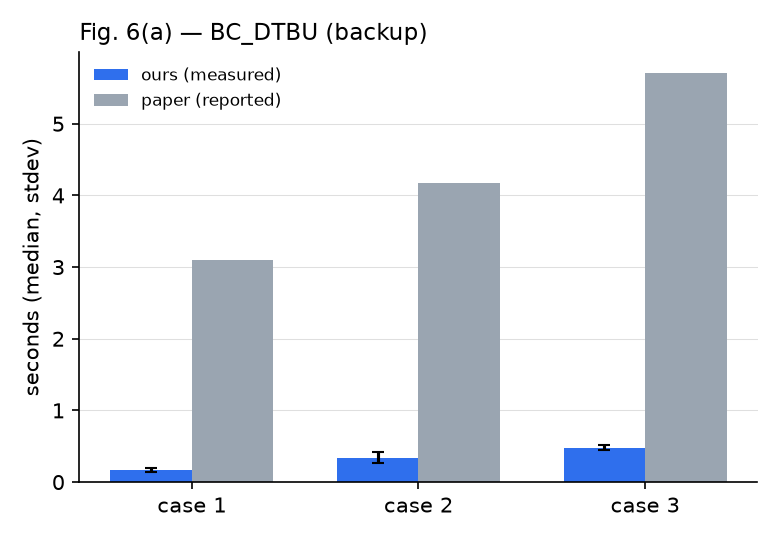
\includegraphics[width=0.49\linewidth]{figs/fig6a_time_backup.png}
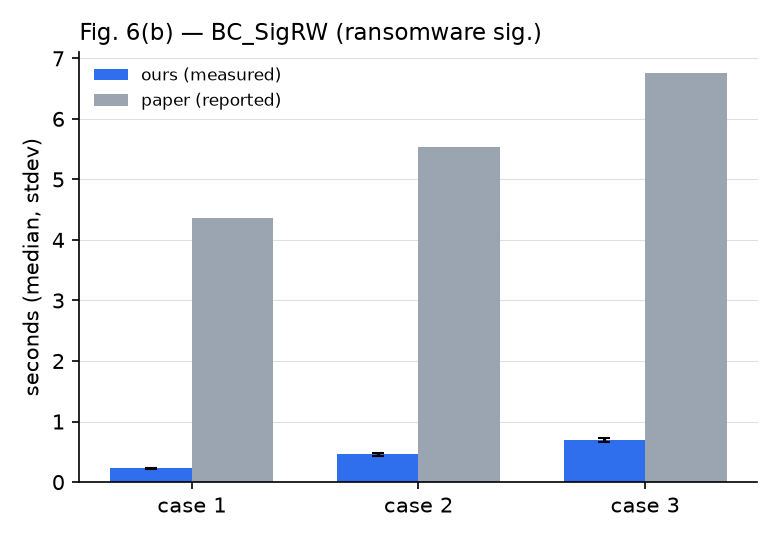
\includegraphics[width=0.49\linewidth]{figs/fig6b_time_ransomware.png}\\[2pt]
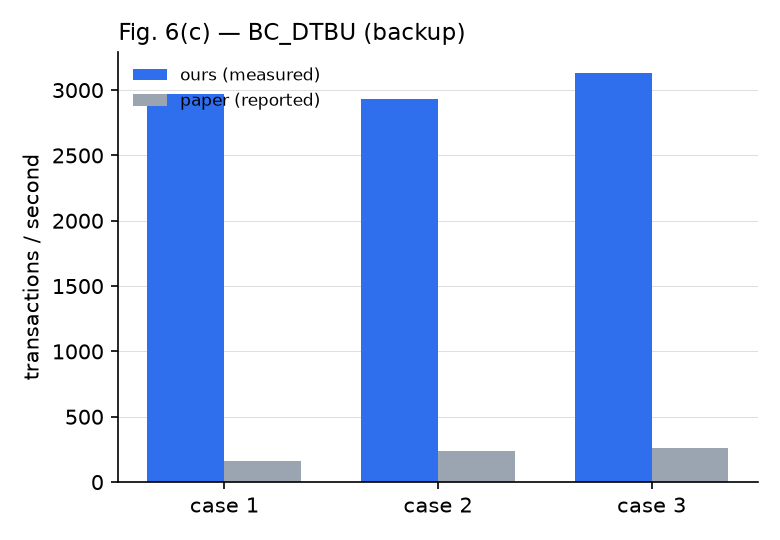
\includegraphics[width=0.49\linewidth]{figs/fig6c_tps_backup.png}
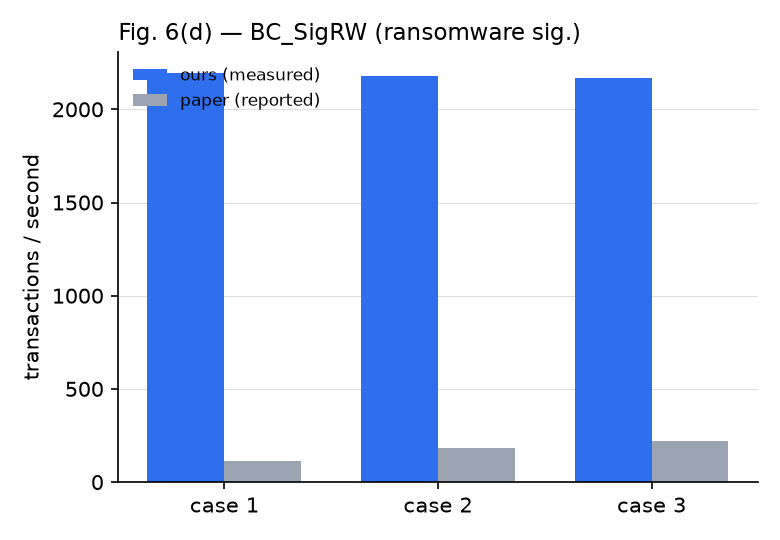
\includegraphics[width=0.49\linewidth]{figs/fig6d_tps_ransomware.png}
\caption{Figs.\ 6(a)--(d) reproductions: measured time and derived TPS, both chains, against the
paper's published values. Our time grows near-linearly with block count rather than
sub-linearly, and our TPS is flat rather than rising -- the direct consequence of the flat
marginal cost in Table~\ref{tab:marginal}.}
\label{fig:timing}
\end{figure}

The paper's headline shape -- time growing sub-linearly, TPS rising as the chain grows -- is not
reproduced. Figure~\ref{fig:timing} shows measured time growing essentially linearly with block
count on both chains, and Table~\ref{tab:marginal} makes the reason explicit: our harness starts
each block's timer only after the cluster is already constructed, so no fixed setup cost sits
inside the measured span to amortise. Per-block marginal cost is flat -- within measurement
noise, the same at case 1 (5 blocks committed) as at case 3 (15 blocks committed) -- on both
chains, and TPS is correspondingly flat rather than rising. This is a second, independent line of
evidence for the claim that the paper's own published TPS values equal $\text{tx}/\text{time}$
exactly, verified against all six of its own data points: the first line of evidence is that
arithmetic identity; this one is a measurement of what the same arithmetic looks like once the
fixed cost is structurally excluded from the timed span, and it produces exactly the flat curve
the amortisation account predicts.

$BC_{SigRW}$ is consistently slower than $BC_{DTBU}$, by 35--44\% across the three cases (paper:
18--41\%). We attribute this structurally, not by tuning to match, to one additional ECDSA
signature per transaction -- the honeypot pipeline's \texttt{attestation}
(\S\ref{sec:honeypot}) -- plus a many-small-floats payload encoding that costs more per byte to
canonicalise than the backup chain's single opaque byte blob.

\subsection{Supplementary: timing under honest, serialization-on conditions}
\label{sec:d3-supplement}

Tables~\ref{tab:timing} and~\ref{tab:marginal} measure consensus with message serialization off --
the M6a run's original configuration. D3 (\texttt{docs/DEVIATIONS.md} DEV-30) found that turning
consensus message serialization on --
every \texttt{Proposal}/\texttt{Prepare}/\texttt{Commit} paying a real encode/decode round-trip,
not the in-memory Python objects the unserialized bus passes -- adds +48--68\% at case-3. Before
presenting the tables above, or building anything further on them, we re-ran the full three-case,
both-chain matrix with serialization on, at the same seed and the same adaptive repeat-count
protocol Table~\ref{tab:timing} uses.

\begin{table}[t]
\centering
\caption{Target 3/4, serialization ON (\texttt{configs/bench.yaml}
\texttt{network.serialize\_messages: true}), same seed and protocol as Table~\ref{tab:timing}.
$\Delta$ is the increase over the serialization-off measurement in that table.}
\label{tab:timing-serialized}
\footnotesize
\begin{tabular}{lccc}
\hline
\textbf{Case / chain} & \textbf{Time (serialized)} & \textbf{$\Delta$ vs.\ Table~\ref{tab:timing}} & \textbf{TPS} \\
\hline
Case 1, $BC_{DTBU}$  & 0.271\,s & +60.9\% & 1848 \\
Case 1, $BC_{SigRW}$ & 0.340\,s & +49.4\% & 1470 \\
Case 2, $BC_{DTBU}$  & 0.544\,s & +59.3\% & 1839 \\
Case 2, $BC_{SigRW}$ & 0.677\,s & +47.6\% & 1476 \\
Case 3, $BC_{DTBU}$  & 0.819\,s & +71.0\% & 1832 \\
Case 3, $BC_{SigRW}$ & 1.043\,s & +50.8\% & 1438 \\
\hline
\end{tabular}
\end{table}

Three questions this answers. \textbf{Does marginal cost stay flat?} Yes -- DEV-08 survives
unchanged: $BC_{DTBU}$ 0.0541--0.0543\,s/block and $BC_{SigRW}$ 0.0678--0.0688\,s/block across
cases 1--3, each varying under 1\%, same shape as serialization-off, just uniformly higher.
Serialization is a per-message cost, not a per-block-count-dependent one, so it cannot
reintroduce the fixed-cost-amortisation shape DEV-08 already ruled out. \textbf{Does the
$BC_{SigRW}$/$BC_{DTBU}$ gap stay at 35--45\%?} No -- it narrows to $\sim$25--27\% (case 1
+25.8\%, case 2 +24.6\%, case 3 +27.4\%). Both chains' D3 encode cost is nearly identical in
absolute terms (0.000072\,s vs.\ 0.000073\,s per block at case 3), so the real bus's fuller
encode+decode cost is plausibly close to chain-independent in absolute seconds; added to
$BC_{DTBU}$'s smaller base, it inflates $BC_{DTBU}$'s own time by a larger percentage than it
inflates the gap, which is why the percentage gap shrinks even as the absolute-seconds gap
grows slightly. This does not overturn the structural ECDSA/encoding attribution above -- that
attribution is specifically about the serialization-off condition, and the serialization-off
35--45\% figure is unchanged -- but any future citation of ``the gap'' must now say which
condition it is under. \textbf{Do the trends still hold?} Yes, on every axis checked: monotone
increase, $BC_{SigRW}$ slower than $BC_{DTBU}$ (narrower, never inverting), and TPS flat rather
than rising, just at a uniformly lower level than Table~\ref{tab:timing}.

\section{Critique}
\label{sec:critique}

Five defects, ordered by severity rather than by the order we found them. They are the ones
that rise to a methodological or architectural problem; a complete record of every smaller
departure from the paper's published design, each with its own rationale, is maintained
separately and is not reproduced here.

\subsection{FLAW-2 -- framework/evaluation disconnect}
\label{sec:flaw2}

Algorithm 2 collects data from a ransomware honeypot and Algorithm 3 trains a detector on the
resulting signatures and behavioural features -- properties of an executing, or emulated,
program. Section VII then evaluates entirely on BitcoinHeist: address-level graph features
(length, weight, count, looped, neighbours, income) of a Bitcoin address that has already
received a ransom payment. These are different problems. Detecting a running ransomware program
from its behaviour and forensically labelling a wallet address after the fact share no features,
no data-generating process, and arguably not even the same notion of a positive instance -- one
is prospective and behavioural, the other retrospective and financial. Nothing in \S IV-C or
\S VII acknowledges the substitution.

We built both pipelines rather than choosing one. The BitcoinHeist pipeline
(\S\ref{sec:5a}--\S\ref{sec:5b}) reproduces the paper's actual published evaluation. The
honeypot pipeline (\S\ref{sec:honeypot}, \S\ref{sec:honeypot-eval}) runs Algorithm 2's honeypot
output through real Phase-2 consensus onto $BC_{SigRW}$, decrypts it back out, and trains
Algorithm 3's four models on it -- the sequence the paper's own Fig.~3 draws. It produces a
real, bounded result (0.8422 balanced accuracy, \S\ref{sec:honeypot-eval}). The paper's
framework half, run end to end as specified, was never demonstrated by its authors; only the
mismatched evaluation half was. FLAW-2 is therefore sharper than ``the paper evaluates on the
wrong data'': the paper's own framework, when actually built and run, produces a defensible
result that the paper itself never reports, choosing an unrelated dataset instead.

\subsection{FLAW-4 -- evaluation methodology}

Section VII resamples BitcoinHeist to 90\% ransomware before evaluating, without stating that the
resample is bounded by the scarce class: only 41{,}413 ransomware rows exist in the cited
2{,}916{,}697-row dataset, so a 90\%-ransomware sample can hold at most
$41{,}413/0.9=46{,}014$ rows -- 1.6\% of the dataset described two paragraphs earlier. The
published 98.98\% accuracy is a number from a $\sim$46K-row experiment, reported with nothing to
mark that it is not the 2.9M-row one. Compounding this, the resulting class balance makes
accuracy nearly free: a constant-positive classifier on this split scores 90.0\%
(\S\ref{sec:5a}).

Reproducing the paper's own protocol exactly, our best model reaches 0.9442/0.9697, 4.56 accuracy
points under published. An ablation over the two candidate leakage sources we could identify --
\texttt{address} retained as a feature, and a non-grouped split -- narrows this only to 3.58
points at the single most leakage-favourable cell tested (Table~\ref{tab:q10}), and both effects
vanish or shrink under the methodologically correct grouped split. We report the residual gap as
unexplained, with a measured bound, rather than attribute it to a cause we found no evidence for.

\subsection{FLAW-5 -- the \S V-3 security claim}
\label{sec:flaw5}

Section V-3 argues that BSFR-SH resists 51\% attacks because it replaces proof-of-work with pBFT.
The argument borrows PoW's 51\% threshold and applies it to a consensus mechanism with a
different one: pBFT is safe only while fewer than $n/3$ of replicas are Byzantine
($n\geq3f+1$). Moving from PoW to pBFT does not raise the fraction of the network an adversary
must control -- it \emph{lowers} it, from just over one half to one third. At the paper's own
deployment of four miner nodes, $f=1$: two colluding replicas (50\% of the cluster -- above the
$f=1$ bound the cluster actually tolerates, and below the 51\% figure the paper cites as the
threshold being defended against) can make two honest replicas commit different blocks at the
same height. We demonstrate this directly rather than argue it: a test constructs exactly this
scenario against our own pBFT implementation and asserts the fork occurs, at exactly the bound
$f$ predicts and no tighter.

The fair counter-argument, which \S V-3 could have made and does not, is that pBFT's threshold
counts identities, not hash power, and in a permissioned deployment identities cannot be minted
by an outside adversary -- a property we test separately, showing a swarm of unauthorised
identities cannot form a certificate regardless of size. The defensible version of \S V-3's claim
is therefore \emph{operational} -- ``an attacker must compromise two of our four named cloud
servers'' -- not consensus-theoretic, and it gets \emph{weaker}, not stronger, in relative terms
as a reason to prefer pBFT over PoW at a fixed and small node count.

\subsection{DEV-26 -- preprocessing deletes the positive class}
\label{sec:flaw-preprocess}

Algorithm 2 line 3 pre-processes honeypot data and, in its entirety, ``removes the
abnormalities.'' The literal reading is statistical outlier removal. On a corpus whose purpose is
teaching a detector what ransomware looks like, that reading is self-defeating: ransomware
behaviour is the minority class by construction -- it \emph{is} the abnormality -- so an
outlier-removal step deletes exactly the samples the detector exists to learn from. Applied
naively, Algorithm 2's own pre-processing step would hand Algorithm 3 a clean-looking dataset
with the positive class silently gone, and \S VII would then report a plausible-looking accuracy
computed on data that never saw an attack. We interpret ``abnormalities'' as sensor defects
rather than unusual behaviour (\S\ref{sec:preprocessing}) and pin the alternative reading's
failure mode with a direct test asserting that cleaning never removes the positive class.

\subsection{DEV-08 -- TPS is amortisation, not throughput}

Section VII-D presents TPS as a measured throughput property that improves as the chain grows
across the paper's three cases. Every one of the six published TPS values equals
$\text{total\_tx}/\text{total\_time}$ exactly, verified to four significant figures against all
six points; the rise the paper reports is the amortisation of a fixed per-run setup cost over a
growing number of blocks, not a throughput property of the consensus mechanism. We add a second,
measured line of evidence beyond this arithmetic observation: when we time only the append span
itself, excluding cluster setup, our own marginal per-block cost is flat across cases 1 through 3
on both chains (Table~\ref{tab:marginal}), and our own TPS is correspondingly flat rather than
rising (\S\ref{sec:5c}). Removing the fixed cost from the timed span removes the rise -- exactly
what ``the rise is amortisation'' predicts, and what our own implementation lets us test
directly rather than infer.

\subsection{GAP-2 -- storage-cost analysis}
\label{sec:storage}

Section VII benchmarks consensus timing but never asks how much storage its own design consumes,
or at what scale that stops being feasible. We compute this from values already measured
elsewhere in this project -- the declared 4096B transaction payload (DEV-15), the measured 215B
framing and 161B hybrid-encryption overhead per chunk (DEV-24), and the measured 1.14$\times$
full-block overhead factor (header, Merkle root and canonical encoding, amortised over a 100-tx
block, \S\ref{sec:5c}) -- rather than from new estimates; full arithmetic in
\texttt{docs/STORAGE\_ANALYSIS.md}.

\begin{table*}[t]
\centering
\caption{On-chain storage growth, daily 1~MiB backups, 4 replicas. Every figure is arithmetic
over \S\ref{sec:5c}'s measured overhead factor, not a new measurement.}
\label{tab:storage}
\footnotesize
\begin{tabular}{lccc}
\hline
\textbf{Scenario} & \textbf{Per-node/yr} & \textbf{Cluster/yr ($\times$4)} & \textbf{Time to 1~TiB/node} \\
\hline
Small clinic (50 pts) & 20.3~GiB & 81.3~GiB & $\approx$50.4~yr \\
Medium hospital (5{,}000 pts) & 1.98~TiB & 7.94~TiB & $\approx$6.05~mo \\
Large network (50{,}000 pts) & 19.8~TiB & 79.4~TiB & $\approx$18.4~days \\
\hline
\end{tabular}
\end{table*}

At hospital scale, the paper's own on-chain design fills 1~TiB per replica in about six months
under daily backups; at network scale, in under three weeks. Backup frequency is the larger lever
of the two the paper leaves open: at the medium scenario, daily backups cost $\approx$7$\times$
weekly and $\approx$30$\times$ monthly in chain growth for identical clinical content, a bigger
effect than DEV-15's payload-size sweep found from a 16$\times$ range of payload sizes alone.

Against this, an on-chain-hash / off-chain-data design -- store only a content digest and a
storage pointer on-chain, keep the encrypted payload in external storage -- preserves the same
tamper-evidence the paper's Merkle-root-and-signature chain already provides (recomputing and
comparing the digest catches off-chain tampering exactly as the paper's own immutability argument
requires), at $\approx$504~bytes per backup regardless of payload size, against
$\approx$1.14~MiB for a 1~MiB backup under the paper's design -- a $\approx$2{,}371$\times$
reduction that widens further as backups get larger, since the hash-only cost is flat and the
paper's is not. What it does not preserve is on-chain \emph{availability}: lose the off-chain
store and the digest alone cannot reconstruct the backup, where the paper's design always can.
We state this trade-off rather than resolving it, per this project's rule against silently
revising the paper's design.

Compute is not the bottleneck this analysis surfaces: the large-network scenario's daily block
count, at \S\ref{sec:5c}'s measured marginal per-block cost, comes to $\approx$4{,}045
CPU-seconds/day ($\approx$4.7\% of a day) on the same 8~GB dev laptop -- comfortably inside its
measured throughput ceiling, though nothing here measures a production cluster's network or disk
behaviour, only this one machine's compute.

\subsection{What the paper gets right}

Two of the paper's choices are execution defects, not premise defects, and the distinction
matters for how it should be read. The two-chain architecture -- one chain for the ground truth a
detector trains on, a separate chain for the backups a system restores from, never sharing node
sets or state -- genuinely does separate detection integrity from recovery integrity: an
adversary who compromises the mechanism protecting one does not thereby compromise the other. And
the central idea that blockchain immutability can protect a detector's training data from
tampering, in a domain where an attacker has every incentive to poison exactly that data if they
can reach it, is sound, and is not the load-bearing idea of any of the four papers Table~II
compares against. The paper's execution of that idea -- its evaluation methodology, its security
argument for choosing pBFT, its preprocessing specification, and the connection between what it
builds and what it measures -- has the five gaps above. Both are true, and a critique that lists
only the five would misrepresent the paper's contribution as smaller than it is.

\section{Honeypot Detection Evaluation}
\label{sec:honeypot-eval}

\S\ref{sec:honeypot} described the design of the honeypot feature pipeline the paper omits. This
section reports what it measures once built end to end: honeypot deployment $\to$ Phase-2
collection $\to$ real four-node pBFT consensus onto $BC_{SigRW}$ $\to$ Phase-3 decryption,
training, and detection -- the sequence Fig.~3 of the paper draws and the paper's own evaluation
never runs.

\begin{table}[t]
\centering
\caption{Honeypot detection result (Alg.\ 3 end to end) and its derived confusion matrix. TP/FP
are computed from the reported precision, recall and evaluation-set composition (353 of 731 eval
records positive) -- a computed quantity, not a separately measured one.}
\label{tab:honeypot}
\footnotesize
\begin{tabular}{lc}
\hline
Train $n$ / Eval $n$ & 1467 / 731 \\
Balanced accuracy & \textbf{0.8422} \\
Precision & 0.8439 \\
Recall & 0.8272 \\
MCC & 0.6849 \\
PR-AUC & 0.9100 \\
Constant-positive baseline & 0.5000 \\
\hline
\multicolumn{2}{c}{\textit{Derived confusion matrix, eval set ($n=731$)}} \\
\hline
True positive & 292 \\
False negative & 61 \\
False positive & 54 \\
True negative & 324 \\
\hline
\end{tabular}
\end{table}

Table~\ref{tab:honeypot} reports the result on the committed corpus (1467 training records, 731
evaluation records, drawn from two independent seeds so no latent generator parameter is shared
across the split): \textbf{0.8422 balanced accuracy}, between the measured simple-Gaussian
baseline (0.830) and the corpus's stated intended ceiling ($\approx0.85$, \S\ref{sec:honeypot})
-- above the naive baseline, not above the ceiling that would indicate the classifier is reading
a leak rather than the corpus's designed difficulty. The evaluation script checks this
automatically against a 0.05 leak margin and refuses to record a result that would fail the
check; it did not fire here. The derived confusion matrix shows a detector that is neither
trivially accurate nor degenerate: 292 of 353 ransomware records correctly flagged, 61 missed, 54
benign records misclassified.

This is the first number in this project produced by Phase 2's output feeding Phase 3's input
through the paper's own architecture. It demonstrates that the framework, as specified, is not
merely completable on paper -- once \S IV-B's undefined $Sig_{RW}$/$FT_{RW}$ are actually given a
definition, Algorithms 2 and 3 connect into a working, non-degenerate detection pipeline. This is
the strongest available rebuttal to a reading of FLAW-2 as ``the framework as designed cannot
work'': it can. The paper simply never tried.

\section{Adversarial Robustness of the Honeypot Detector}
\label{sec:adversarial}

\S\ref{sec:honeypot-eval}'s 0.8422/0.8408\footnote{This section trains and evaluates on
\texttt{data/honeypot/corpus\_\{train,eval\}.csv} directly, per \S\ref{sec:honeypot}'s ``committed
corpus is the fixed dataset'' convention. Read this way the same seed and configuration give
0.8408, not 0.8422: \texttt{honeypot/corpus.py} formats every feature to six significant figures
when it writes the CSV, and that rounding alone accounts for the 0.0014 difference from
Table~\ref{tab:honeypot}'s chain-reconstructed, full-precision number. Both are measured; neither
is wrong; every threshold below is relative to 0.8408.} balanced accuracy answers ``does the
detector work.'' It does not answer ``does it keep working against an adversary who knows a
behavioural sensor is watching.'' The paper's threat model is silent on this: Algorithm 3 assumes
$FT_{RW}$ is simply observed, never that a rational attacker -- one motivated to avoid exactly the
detection Algorithm 3 performs -- would adjust their program's observable behaviour to defeat it.
This is not a gap we can hold against the paper alone: testing it requires a defined, differentiable
feature pipeline, which is precisely what \S IV of the paper never provides (FLAW-2). Only having
built $FT_{RW}$ ourselves (DEV-03, DEV-27) makes the question answerable at all.

\begin{table}[t]
\centering
\caption{Top-5 features by Random Forest importance (individually, bal.\ acc.\ 0.8513 on the
committed corpus -- the higher of the two importance-bearing models, Decision Tree scoring
0.8063), with each feature's evasion direction and physical bound.}
\label{tab:top5}
\footnotesize
\begin{tabular}{lccl}
\hline
\textbf{Feature} & \textbf{Importance} & \textbf{Direction} & \textbf{Bound} \\
\hline
observed\_stages & 0.126 & $\downarrow$ & 0 stages \\
extension\_change\_rate & 0.109 & $\downarrow$ & 0 \\
rename\_rate\_per\_s & 0.079 & $\downarrow$ & 0 s$^{-1}$ \\
write\_entropy\_var & 0.074 & $\uparrow$ & 6.5494 \\
crypto\_ngram\_novelty & 0.067 & $\downarrow$ & 0 \\
\hline
\end{tabular}
\end{table}

Table~\ref{tab:top5}'s bounds are not arbitrary. Four features move toward 0 -- an attacker can
always throttle: delay the kill chain so fewer of the four observable stages complete inside a
honeypot's finite dwell time (\texttt{observed\_stages}), rename files less aggressively or not at
all (\texttt{extension\_change\_rate}), slow the rename loop (\texttt{rename\_rate\_per\_s}), or
mimic a common, previously-seen crypto-API call sequence instead of a distinctive one
(\texttt{crypto\_ngram\_novelty}). The fifth, \texttt{write\_entropy\_var}, moves the other way:
ransomware ciphertext is consistently near-maximal entropy (\emph{low} variance across blocks),
while benign writes are heterogeneous, so an attacker raises variance by interleaving some
deliberately low-entropy writes among the ciphertext. Its bound, 6.5494, is not an abstract limit
but the highest \texttt{write\_entropy\_var} the generator's own benign profiles are ever observed
to produce in the committed corpus -- an attacker cannot manufacture more heterogeneity than a
real, non-malicious write pattern in this environment exhibits. No feature in the top-5 turned out
structurally robust (unlike mean write entropy, which cannot fall below the entropy of properly
encrypted data and is exactly the kind of feature that would resist this attack, but did not rank
in the top 5).

\begin{figure}[t]
\centering
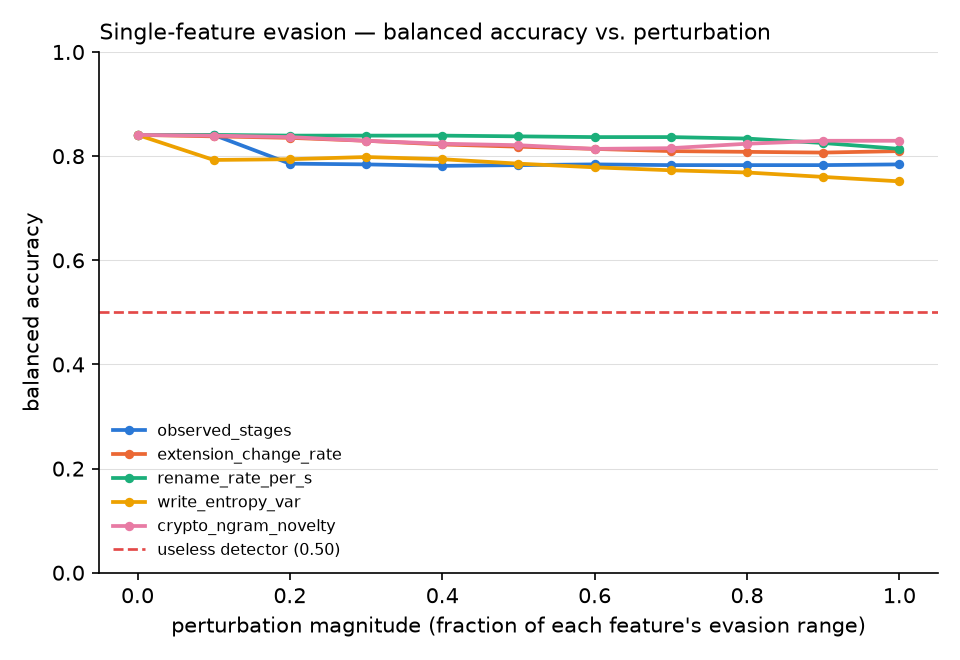
\includegraphics[width=\linewidth]{figs/fig7a_single_feature_degradation.png}
\caption{Each top-5 feature perturbed independently, 0--100\% of its evasion range, against the
committed eval corpus's 353 malicious rows. Ensemble fit once; never retrained.}
\label{fig:single-feature}
\end{figure}

\textbf{Single-feature evasion is weak.} Figure~\ref{fig:single-feature} shows every individual
feature, pushed all the way to its bound, costing the detector at most 9 points of balanced
accuracy (0.841 $\to$ 0.752 for \texttt{write\_entropy\_var}, the largest single-feature drop;
\texttt{rename\_rate\_per\_s} alone costs under 3 points). None approaches 0.50. A one-dimensional
attacker -- one who tunes a single observable behaviour and leaves everything else alone -- does
not meaningfully dent this detector.

\begin{figure}[t]
\centering
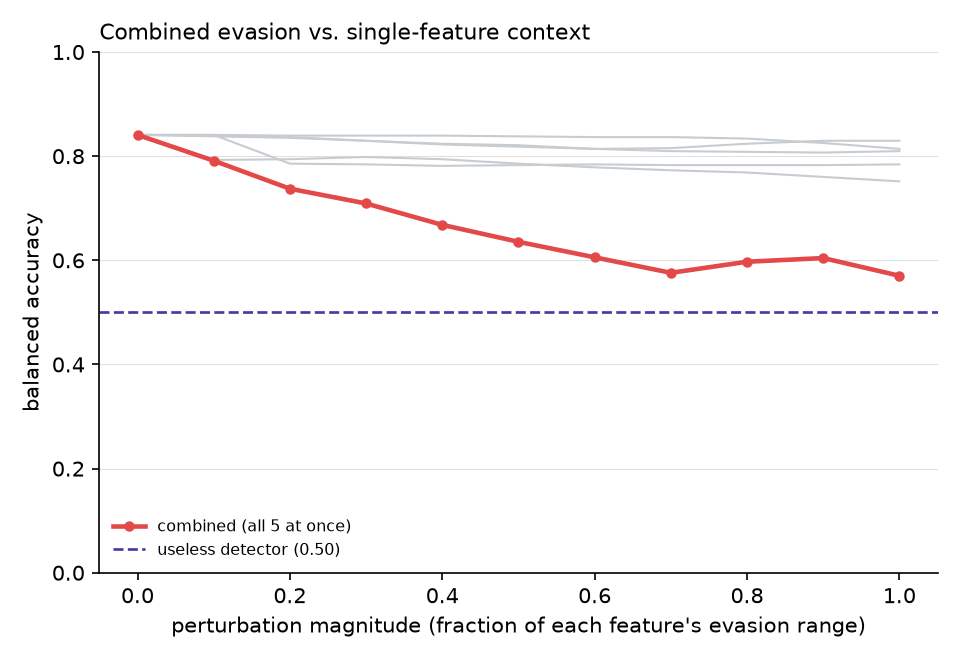
\includegraphics[width=\linewidth]{figs/fig7b_combined_evasion.png}
\caption{All five features perturbed simultaneously (bold), against the five single-feature curves
as context (light gray) on the same axes.}
\label{fig:combined}
\end{figure}

\textbf{Combined evasion compounds, but does not collapse the detector.} Perturbing all five
features together (Figure~\ref{fig:combined}) drops balanced accuracy from 0.841 to a floor
around 0.57--0.60 by 60--100\% joint perturbation -- roughly triple any single feature's damage,
confirming the features compound as a competent adversary would exploit. It never reaches the
0.50 useless-detector line, though: the top-5 features carry only 45.5\% of Random Forest's total
importance mass (0.126+0.109+0.079+0.074+0.067), so the remaining 17 features, entirely
unperturbed here, still carry real discriminative signal even once the five most important ones
are pushed to their physical limits. This is itself the finding -- exactly the outcome the session
brief's own test criterion anticipated as a possibility (``the model uses features outside the
top-5 enough to still discriminate''), and it is a mild point in the detector's favor: no small,
named feature subset is a single point of failure.

\begin{figure}[t]
\centering
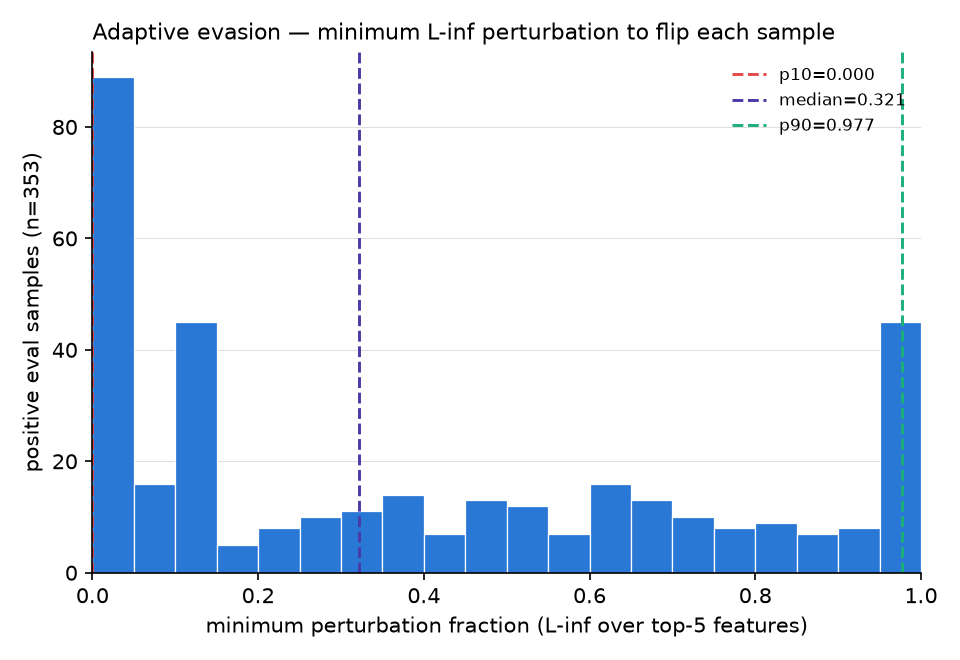
\includegraphics[width=\linewidth]{figs/fig7c_adaptive_evasion_histogram.png}
\caption{Per-sample minimum $L_\infty$ perturbation (top-5 features, each normalized to its own
evasion range) that flips the ensemble's verdict, over all 353 positive eval rows.}
\label{fig:adaptive}
\end{figure}

\textbf{Adaptive, per-sample evasion is a different picture.} An adversary who knows the model and
optimizes per sample does much better than one perturbing blindly. Binary search per positive row
over the $L_\infty$ ball (Figure~\ref{fig:adaptive}) finds: median minimum perturbation
\textbf{0.321} (a typical ransomware sample needs about a third of the available evasion range to
flip); 10th percentile \textbf{0.000} -- driven by the 61 of 353 positive rows (17.3\%) the
detector already misses at 0\% perturbation (consistent with the measured 0.8408's own false-negative
rate), plus a further 7.9\% needing under 5\% perturbation, so roughly a quarter of ransomware
samples are trivially evadable by an adaptive attacker; 90th percentile \textbf{0.977} -- the
hardest samples need nearly the entire evasion range. 28 of 353 positive rows (7.9\%) never flip
even at the full $L_\infty$ ball. Checking those survivors against the sixth-through-tenth ranked
features (never perturbed here) shows exactly what the session's own test criterion predicted:
survivors average \texttt{c2\_beacon\_count} 10.3 against 7.0 for the malicious class as a whole,
\texttt{entropy\_delta} 3.58 against 2.61, and similarly elevated \texttt{key\_generation\_events},
\texttt{shadow\_copy\_deletions} and \texttt{dns\_entropy} -- these are the ransomware samples so
extreme on features outside the top-5 that disguising only the top-5 cannot save them.

\textbf{Conclusion: shape (c), the nuanced answer.} No single top-5 feature is fragile enough to
break the detector alone, and no combination of exactly these five is either -- the ensemble's
reliance on 17 further features is real and measured, not assumed. But a median-effort adaptive
adversary needs only about a third of the physically plausible evasion range, and roughly a
quarter of ransomware samples are evadable with under 5\% perturbation on features an attacker can
freely throttle to zero. The paper's implicit assumption that $FT_{RW}$ is unconditionally robust
is false for a meaningful minority of cases and approximately true for the rest, and this
asymmetry -- some samples essentially free to evade, others requiring near-maximal effort -- is
exactly the kind of result a single aggregate accuracy number cannot show. It is a direct
consequence of FLAW-2 (\S\ref{sec:flaw2}): the paper's own evaluation, run on BitcoinHeist address
features that no attacker can \emph{choose their own value of} at will, could never have surfaced
this question, because it is a question about behavioural features an attacker actually controls.
Only the framework path this project built makes it a question with a measured answer.

\section{Consensus Comparison: pBFT vs.\ Raft}
\label{sec:m7-4}

\S V-3's argument for pBFT (\S\ref{sec:flaw5}) does not survive scrutiny, and once it falls the
paper is left having chosen pBFT without ever asking the question its own deployment invites: four
cloud servers the operator controls are exactly the setting where ``do we actually need Byzantine
fault tolerance?'' is legitimate, because BFT's cost buys protection against a specific threat --
an actively lying node -- that the paper never argues is the one it faces. This section asks that
question directly, against Raft (Ongaro \& Ousterhout), the standard crash-fault-tolerant
alternative: simpler, faster, and covered by the same distributed-systems curriculum (6.5840 Lab
2/3) that motivated implementing it here.

\textbf{What Raft is, briefly.} Raft replicates a log across $n$ replicas via a single elected
leader. Followers accept whatever the current-term leader's \texttt{AppendEntries} tells them,
subject only to a term check and a previous-entry consistency check; the leader declares an entry
committed once a majority of replicas have replicated it, and that fact then propagates via the
next \texttt{AppendEntries}. Leader election uses randomized timeouts and a log-completeness
voting rule so that a new leader is guaranteed to hold every previously committed entry. Unlike
pBFT, no message in the protocol is signed, and no replica ever cross-checks another replica's
copy of an entry -- correctness rests entirely on trusting the current leader.

We implemented Raft (\texttt{consensus/raft.py}) over the identical four-node cluster, message
bus, and \texttt{ClientRequest} submitter-authentication path as pBFT, differing only in the
consensus protocol itself, and made \texttt{framework.\_block\_pipeline} consensus-agnostic
(\texttt{consensus.interface.ConsensusCluster}, DEV-32) so the same pipeline code drives either
cluster. Log compaction, cluster membership changes, and snapshotting are out of scope, matching
the same kind of reduction pBFT's own view-change implementation already accepted (DEV-20).

\subsection{Quantitative: timing, messages, TPS}

\begin{table*}[t]
\centering
\caption{pBFT vs.\ Raft, both chains, all three cases, serialization on (5 repeats, seed 20260924,
run \texttt{20260924T045952Z-2eaa456f}). Messages and signature operations are the median across
repeats of the whole run's totals; timing and TPS as in Table~\ref{tab:timing}.}
\label{tab:m7-4-matrix}
\footnotesize
\begin{tabular}{llccccc}
\hline
\textbf{Case} & \textbf{Chain} & \textbf{Protocol} & \textbf{Time (s)} & \textbf{TPS} &
\textbf{Messages} & \textbf{Sig.\ ops} \\
\hline
1 & $BC_{DTBU}$  & pBFT & 0.2708 & 1846 & 140 & 140 \\
1 & $BC_{DTBU}$  & Raft & 0.2461 & 2032 &  92 &   0 \\
1 & $BC_{SigRW}$ & pBFT & 0.3397 & 1472 & 140 & 140 \\
1 & $BC_{SigRW}$ & Raft & 0.3142 & 1592 &  92 &   0 \\
2 & $BC_{DTBU}$  & pBFT & 0.5490 & 1822 & 280 & 280 \\
2 & $BC_{DTBU}$  & Raft & 0.4923 & 2031 & 172 &   0 \\
2 & $BC_{SigRW}$ & pBFT & 0.6807 & 1469 & 280 & 280 \\
2 & $BC_{SigRW}$ & Raft & 0.6378 & 1568 & 172 &   0 \\
3 & $BC_{DTBU}$  & pBFT & 0.8433 & 1779 & 420 & 420 \\
3 & $BC_{DTBU}$  & Raft & 0.7500 & 2000 & 252 &   0 \\
3 & $BC_{SigRW}$ & pBFT & 1.0230 & 1466 & 420 & 420 \\
3 & $BC_{SigRW}$ & Raft & 0.9483 & 1582 & 252 &   0 \\
\hline
\end{tabular}
\end{table*}

Table~\ref{tab:m7-4-matrix} is the full matrix: cases 1--3, both chains, both protocols,
serialization on (the condition DEV-30 settled M6a's own numbers on). Two structural properties
hold exactly, independent of chain or case:

\begin{itemize}
\item \textbf{Messages are flat per block, at two different levels.} pBFT sends exactly 28
messages per committed block in every case ($140/5=280/10=420/15=28$) -- $O(n^2)$ fan-out
(pre-prepare, prepare, commit, each broadcast) at a fixed $n=4$. Raft converges toward roughly 17
messages per block as the one-time leader-election cost amortises across more blocks
($92/5=18.4$, $172/10=17.2$, $252/15=16.8$) -- $O(n)$ fan-out, plus a second leader-driven
broadcast round to announce the new commit index. At steady state Raft sends about 60\% of pBFT's
message count: a real, measured reduction, but far short of the $O(n^2)$-vs-$O(n)$ asymptotic gap
a much larger cluster would show. $n=4$ is simply too small for the quadratic term to dominate.
\item \textbf{Signature operations are exactly zero for Raft, in every cell.} pBFT signs and
verifies every pre-prepare/prepare/commit; Raft's \texttt{AppendEntries}/\texttt{RequestVote}
carry no signature at all, by design (\texttt{consensus/raft.py}). This is the sharpest, cleanest
number in the table, and it is also the number that most directly costs security -- see
\S\ref{sec:m7-4-byzantine}.
\end{itemize}

\textbf{The timing gap is much smaller than the message-count gap, and that is itself a finding.}
Raft is 7--11\% faster than pBFT across the matrix (e.g.\ case 3, $BC_{DTBU}$: 0.750\,s vs.\
0.843\,s), not the $\sim$40\% the message-count reduction alone might suggest. This is exactly
consistent with DEV-08/DEV-21's existing finding that consensus messaging is a small fraction of
the measured span at zero simulated network delay: hybrid encryption, block construction, and
(with serialization on, DEV-30) message encoding dominate wall-clock time, and shaving a third of
the message count off an already-small component of the total produces a proportionally small
timing change. If the deployment's real bottleneck is cryptographic and encoding work rather than
consensus round trips, switching consensus protocols buys a modest, not a transformative, speedup
-- the timing number the paper never measured turns out to matter less than the message-count
number it never asked about.

\subsection{Qualitative: the Byzantine leader}
\label{sec:m7-4-byzantine}

We ran both protocols with one of four nodes silently crashed and, separately, one of four nodes
byzantine.

\textbf{Crash fault (both protocols): commits continue.} With one node's outgoing messages
dropped from the start, the other three nodes committed every submitted block under both
protocols (\texttt{crash\_tolerance\_pbft}/\texttt{crash\_tolerance\_raft}, run
\texttt{20260924T045952Z-2eaa456f}: all three live replicas reached height 3 of 3 either way).
$n=4$ tolerates one crash under Raft's majority rule exactly as it tolerates one Byzantine replica
under pBFT's $f=1$ -- the same \emph{count} of tolerated failures, a different failure
\emph{model}.

\textbf{Byzantine leader (Raft only): commits continue, on different data.} We installed a
behaviour on Raft's elected leader that sends genuinely different, honestly-signed transaction
sets to different followers at the same log index, each claiming the entry is already committed
-- standard, protocol-compliant \texttt{AppendEntries} on both sides, no forged signature and no
bug in either sender or receiver. Every node ``committed'' by its own local rule: all four reached
height 2, but two followers hold block hash
\texttt{ebd2c097fd90b599\ldots} while the third holds \texttt{a6cf98b3bdd0447e\ldots} -- two
different, individually valid, individually well-linked blocks at one height
(\texttt{raft\_byzantine\_fork}, same run; reproduced as a standing regression test in
\texttt{tests/unit/test\_raft\_byzantine.py}). Neither side's chain integrity check catches this,
because both blocks are genuinely well-formed; the check that would catch it -- cross-referencing
what a majority of \emph{other} replicas independently attest to -- is exactly the check pBFT's
$2f+1$ matching-vote quorum performs and Raft's leader-trust model does not.

pBFT resists the equivalent attempt structurally: two followers committing different content at
one height would require $2f+1$ matching votes for \emph{each} side, which needs more faulty
replicas than $f=1$ permits at $n=4$ (\S\ref{sec:flaw5} already demonstrates the actual threshold
is two colluding replicas, not one).

\subsection{The trade-off, stated precisely}

Raft is 7--11\% faster and sends roughly 60\% as many consensus messages as pBFT at this cluster
size, but a single compromised leader corrupts the chain undetectably -- every node individually
believes consensus succeeded, and nothing in Raft's protocol or in \texttt{Chain}'s own validation
(Merkle root, signature, linkage) notices the fork. Whether that trade-off is acceptable depends
entirely on whether the deployment's threat model includes active server compromise, not merely
server failure -- a question \S V-3 never asks, because it substitutes a borrowed 51\% figure for
an actual threat-model argument (\S\ref{sec:flaw5}). For a smart-healthcare deployment whose own
threat model (\S II) explicitly includes a compromised or malicious cloud server, that gap is not
a minor implementation detail: it is the entire reason pBFT, not Raft, is the correct choice here
-- but it is a reason the paper never states, and the 7--11\% speed cost of stating it and paying
for it honestly is modest.

\section{Hybrid Blockchain}
\label{sec:hybrid}

\S VIII of the paper itself states its own limitation and stops: ``in future, we have plan to
work with hybrid blockchain.'' No design follows. \S IV-A already names the trade-off this answers
without resolving it: a private, permissioned chain is fast and keeps healthcare data
confidential, but its integrity rests entirely on trusting the four cloud servers that operate
it -- nothing in the paper's design lets anyone outside that set confirm $BC_{DTBU}$ or
$BC_{SigRW}$ have not been silently rewritten. A public chain would give that external
verifiability, at the cost of exposing whatever it carries to everyone. A hybrid design keeps the
paper's own private chains exactly as built -- same speed, same confidentiality, \S IV's pBFT
consensus unchanged -- and adds one small, public commitment alongside them.

\subsection{Architecture: an anchor chain and the \texttt{AnchorRecord} schema}

An \texttt{AnchorRecord} carries one private block's height, its header hash $HC_{\beta_j}$, its
Merkle root $MTR$, a timestamp, and the anchor creator's ECDSA signature over all of it -- copied
verbatim from the private block's own header, never derived from, or requiring decryption of, its
transactions. Every other transaction in this codebase is $E_{KU_{CS_l}}(Tx)$ (Alg.~1 line~2 /
Alg.~2 line~7), sealed so only one cloud server can read it; an anchor record inverts that
deliberately -- its only job is to be readable by anyone, so it is never encrypted.

The anchor chain is simulated, not real Ethereum or Bitcoin, and is modelled as a second,
independent \texttt{Chain} instance with its own consensus. That consensus is direct
sign-and-append by a single authority, not a second pBFT cluster: a single signer has no other
replica to convince, so pBFT's message rounds would be pure overhead with nothing underneath them.
This was a correction, not the first design -- an earlier version ran the anchor chain through a
literal single-node pBFT cluster, which worked, but pulled a dependency from the blockchain layer
up into consensus/framework code that this project's own architectural boundary (enforced by a
standing test, not merely documented) correctly rejected. The point of the exercise was always the
\emph{interface} a hybrid chain needs from its anchor -- commit, and answer whether a given block
still matches what was committed -- not the anchor's own Byzantine fault tolerance, which a real
public chain supplies for itself. Full rationale in \texttt{docs/DEVIATIONS.md} DEV-33.

Given an anchor record and a candidate block claiming to be the one it covers, anyone can check
its hash and Merkle root against the record without decrypting a single transaction inside it.
That is the whole guarantee: the private chain's shape at that height is fixed the moment the
anchor commits, even against an operator who controls every private-chain replica. It is not a
claim about the private chain's contents being correct -- only that they cannot change afterward
without the change being visible to anyone holding the anchor.

\subsection{The anchor frequency trade-off}

\texttt{AnchorPolicy.frequency} is the cost/integrity lever: anchoring every block gives maximum
integrity at maximum anchor traffic; anchoring every $N$th block cuts that traffic by $N\times$ at
the cost of up to $N{-}1$ blocks' unanchored tampering window. Table~\ref{tab:m7-5-matrix} sweeps
$N \in \{1, 5, 10\}$ across the paper's own three cases, both chains, serialization on -- the same
condition \S VIII's comparison settled on.

\begin{table*}[t]
\centering
\caption{Hybrid vs.\ private-only, both chains, all three cases, anchor frequency 1/5/10,
serialization on (5 repeats, seed 20260925, run \texttt{20260924T213216Z-2bd78940}). Hybrid
seconds is the identical private commit plus one \texttt{sync()}+\texttt{flush()} pair.}
\label{tab:m7-5-matrix}
\footnotesize
\begin{tabular}{llccccc}
\hline
\textbf{Case} & \textbf{Chain} & \textbf{Freq} & \textbf{Private (s)} & \textbf{Hybrid (s)} &
\textbf{Overhead} & \textbf{Anchors (bytes)} \\
\hline
1 & $BC_{DTBU}$  & 1  & 0.27387 & 0.27287 & $-0.37\%$ & 5 (5029) \\
1 & $BC_{DTBU}$  & 5  & 0.27387 & 0.27372 & $-0.05\%$ & 1 (1004) \\
1 & $BC_{DTBU}$  & 10 & 0.27387 & 0.27419 & $+0.12\%$ & 1 (1004) \\
1 & $BC_{SigRW}$ & 1  & 0.33973 & 0.33887 & $-0.25\%$ & 5 (5035) \\
1 & $BC_{SigRW}$ & 5  & 0.33973 & 0.33673 & $-0.88\%$ & 1 (1006) \\
1 & $BC_{SigRW}$ & 10 & 0.33973 & 0.33907 & $-0.19\%$ & 1 (1005) \\
2 & $BC_{DTBU}$  & 1  & 0.54432 & 0.54371 & $-0.11\%$ & 10 (10060) \\
2 & $BC_{DTBU}$  & 5  & 0.54432 & 0.54329 & $-0.19\%$ & 2 (2013) \\
2 & $BC_{DTBU}$  & 10 & 0.54432 & 0.54137 & $-0.54\%$ & 1 (1009) \\
2 & $BC_{SigRW}$ & 1  & 0.67989 & 0.68087 & $+0.14\%$ & 10 (10077) \\
2 & $BC_{SigRW}$ & 5  & 0.67989 & 0.67193 & $-1.17\%$ & 2 (2021) \\
2 & $BC_{SigRW}$ & 10 & 0.67989 & 0.74360 & $+9.37\%$ & 1 (1009) \\
3 & $BC_{DTBU}$  & 1  & 0.81568 & 0.81811 & $+0.30\%$ & 15 (15105) \\
3 & $BC_{DTBU}$  & 5  & 0.81568 & 0.91398 & $+12.05\%$ & 3 (3018) \\
3 & $BC_{DTBU}$  & 10 & 0.81568 & 0.86512 & $+6.06\%$ & 2 (2016) \\
3 & $BC_{SigRW}$ & 1  & 1.01988 & 1.03381 & $+1.37\%$ & 15 (15131) \\
3 & $BC_{SigRW}$ & 5  & 1.01988 & 1.01789 & $-0.20\%$ & 3 (3027) \\
3 & $BC_{SigRW}$ & 10 & 1.01988 & 1.02178 & $+0.19\%$ & 2 (2019) \\
\hline
\end{tabular}
\end{table*}

Two findings, both against the frequency lever's intuition. First, anchor overhead is at or below
measurement noise, not a real structural cost: 15 of 18 cells fall within $\pm 1.4\%$, and the
three outliers ($+9.37\%$, $+12.05\%$, $+6.06\%$) do not track with frequency or chain in any
consistent direction -- the signature of scheduling jitter between two separately built clusters,
not a per-anchor cost, and expected given \texttt{sync()}/\texttt{flush()} runs no consensus at
all. Second, anchor chain storage is tiny and flat: every anchor costs
$\approx$1.00--1.01\,KB regardless of case or chain (5029/5, 10060/10, 15105/15 bytes-per-anchor
all $\approx$1006), because an \texttt{AnchorRecord} is two 32-byte hashes plus fixed-size
metadata, never a function of the private block's own payload size. The frequency lever therefore
trades anchor count linearly against the tampering window it leaves open, not against a real
cost curve on the anchor side -- the anchor's own cost is already negligible at $N{=}1$.

\subsection{What external verifiability buys: three security tests}

Three tests, mirroring \texttt{tests/unit/test\_hybrid\_chain.py}, demonstrate what the anchor
adds and where it honestly does not reach.

\textbf{(a) Tamper a private block after it is anchored.} A private-chain block already covered by
an \texttt{AnchorRecord} is replaced, on every replica, by a different, internally
well-formed, validly-signed block at the same height -- the same class of attack \S VIII's
Byzantine-leader test constructs, applied here to storage rather than to consensus.
\texttt{verify\_anchor} recomputes the live block's hash and Merkle root on every call and compares
them against the stored record: \texttt{anchored=True, verified=False}. The tamper is caught.

\textbf{(b) Tamper a private block that has not been anchored yet.} At frequency $N{=}5$, heights
6 and 7 of a 7-block chain are not covered by any anchor until a later multiple or a flush closes
the window. Tampering height 6 in that gap produces \texttt{anchored=False}: there is nothing to
check it against, so nothing is claimed either way. This is stated as the honest cost of
infrequent anchoring, not smoothed over -- it is exactly the $N{-}1$-block tampering window named
above as the trade-off's price, demonstrated rather than assumed.

\textbf{(c) Tamper the anchor chain itself.} The anchor chain's own stored blocks are replaced the
same way as in (a). \texttt{verify\_anchor\_chain\_integrity} -- \texttt{Chain.verify\_integrity},
unmodified, applied to the anchor chain -- catches the broken link and the invalid signature, the
same way it would for either private chain. This catches storage-level tampering of the anchor
chain, but rests on an assumption stated plainly rather than hidden: it does not model an attacker
who controls the anchor authority's own signing key from the start. In production the anchor chain
is a real public blockchain with its own, separate consensus; an operator who also controlled that
consensus would defeat the entire hybrid design, not just this check.

\subsection{Limitations, stated honestly}

The anchor chain here is simulated, and three simplifications matter for anyone reading these
numbers as evidence about a real deployment. First, a real public chain (Ethereum, Bitcoin, or a
purpose-built one) has real network latency and a real per-transaction cost -- gas fees on
Ethereum, most concretely -- neither of which this simulation pays; the $\approx$1\,KB/anchor
figure above is a storage cost, not a gas estimate, and the two do not convert directly. Second,
this simulation's anchor authority is a single signing key with no consensus of its own; a real
deployment anchoring to a public chain submits one signed transaction per anchor to that chain's
own, already-running consensus, which is a fair analogue of what is modelled here, but the
public chain's own liveness and finality guarantees are not exercised by anything in this section.
Third, and most fundamentally, the paper's threat model (\S II) never specifies who the external
verifier actually is -- a regulator, a patient, an independent security researcher auditing the
deployment -- and this design does not pick one either. What it provides is that verification is
possible for any of them without a relationship with the private chain's operators, which is the
property \S IV-A's trade-off was missing; deciding who should exercise it is a policy question
this report does not answer.

\section{Conclusion}

We built a complete, from-scratch implementation of BSFR-SH's five algorithms, both of its
independent private blockchains under real pBFT consensus, and both a faithful reproduction of
the paper's published evaluation and the honeypot feature pipeline its own Phase 2/3 requires but
never defines. Reproducing the paper's own methodology exactly, its headline detection result
does not reproduce: our best model reaches 0.9442/0.9697 against a published 0.9898/0.990, and an
ablation over both candidate leakage sources we identified narrows but does not close a
3.58-point residual gap. We find five further, independent defects -- a disconnect between what the
framework is designed to detect and what it is evaluated on, a degenerate and undisclosed
evaluation split, a security argument that inverts pBFT's actual threshold relative to
proof-of-work, a preprocessing specification that, read literally, deletes the class it exists to
detect, and a reported throughput curve that is arithmetic amortisation rather than a measured
property. Against this, the paper's central architectural idea -- two chains, separately
protecting a detector's ground truth and a system's recoverability, from an adversary with every
incentive to attack both -- is sound, and our own honeypot pipeline shows the framework can
produce a real, bounded detection result (0.8422 balanced accuracy) once its undefined layer is
actually built.

What remains open: the 3.58-point gap between our best reproduction and the published figure has
a measured lower bound but no identified cause -- neither address-as-feature nor split strategy,
alone or together, explains it, and no further candidate was tested for lack of one. Of the five
stretch extensions the project roadmap identified, four are built and reported above: a formal
(Scyther) model of the session-establishment protocol (\S III-B), a storage-cost analysis for
on-chain healthcare backups at realistic scale (\S V-F), adversarial feature-space evasion against
the detector (\S VII), and a comparison against Raft as an alternative consensus protocol
(\S VIII). A fifth, hybrid-blockchain support, is reported in \S IX, directly answering \S VIII of
the paper itself, which names it as its own future work. One extension remains unpursued: an
asynchronous pBFT variant with modelled network latency beyond the fixed delays
\S IV-C already sweeps.

Taken together, the two findings point in the same direction rather than opposite ones. A paper
whose evaluation methodology cannot be checked because its protocol is underspecified, and whose
one checkable headline number does not reproduce even under the most literal reading of its own
stated split, is a paper whose central empirical claim should not be relied on as published. That
is a narrower conclusion than ``the framework does not work'': our own honeypot pipeline shows a
version of Algorithm 3, trained on data Algorithm 2 actually specifies producing, detecting
ransomware at a real, bounded, non-degenerate rate. The architecture is worth building on. The
published numbers, as published, are not evidence that it works as well as claimed.

\begin{thebibliography}{9}

\bibitem{wazid2023}
M.~Wazid, A.~K.~Das, and S.~Shetty, ``BSFR-SH: Blockchain-Enabled Security Framework Against
Ransomware Attacks for Smart Healthcare,'' \emph{IEEE Trans.\ Consumer Electronics}, vol.~69,
no.~1, pp.~18--28, Feb.\ 2023.

\bibitem{castro-liskov}
M.~Castro and B.~Liskov, ``Practical Byzantine Fault Tolerance,'' in \emph{Proc.\ 3rd USENIX
Symp.\ Operating Systems Design and Implementation (OSDI)}, 1999.

\bibitem{akcora2021bitcoinheist}
C.~G.~Akcora, Y.~Li, Y.~R.~Gel, and M.~Kantarcioglu, ``BitcoinHeist: Topological Data Analysis
for Ransomware Prediction,'' \emph{IJCAI}, 2021 (BitcoinHeist Ransomware Address Dataset, UCI
Machine Learning Repository; cited in \cite{wazid2023} as ref.~[15]).

\bibitem{almashhadani}
A.~Almashhadani \emph{et al.}, network-traffic-based ransomware detector evaluated on Locky
traffic traces, \emph{IEEE Access}, vol.~7, 2019; cited in \cite{wazid2023} as ref.~[11].

\bibitem{hwang}
J.~Hwang \emph{et al.}, dynamic-analysis-based ransomware detector, \emph{Wireless Personal
Communications}, vol.~112, 2020; cited in \cite{wazid2023} as ref.~[12].

\bibitem{sharmeen}
S.~Sharmeen \emph{et al.}, semi-supervised ransomware detector evaluated on an independent
corpus, \emph{IEEE Access}, vol.~8, 2020; cited in \cite{wazid2023} as ref.~[13].

\bibitem{bae}
S.~I.~Bae \emph{et al.}, PE-file-feature-based ransomware detector, \emph{Concurrency and
Computation: Practice and Experience}, vol.~32, 2020; cited in \cite{wazid2023} as ref.~[14].

\bibitem{rfc6979}
T.~Pornin, ``Deterministic Usage of the Digital Signature Algorithm (DSA) and Elliptic Curve
Digital Signature Algorithm (ECDSA),'' RFC~6979, IETF, Aug.\ 2013.

\bibitem{cremers2008scyther}
C.~Cremers, ``The Scyther Tool: Verification, Falsification, and Analysis of Security
Protocols,'' in \emph{Computer Aided Verification (CAV)}, LNCS vol.~5123, Springer, 2008,
pp.~414--418.

\end{thebibliography}

\end{document}
